\section*{Task 6}

\begin{figure}[H]
\centering
\begin{circuitikz}[american voltages]

    \node[circle, fill=black, inner sep=0pt] (TL) at (-5, 2) {};
    \node[circle, fill=black, inner sep=0pt] (TM) at (1, 2) {};
    \node[circle, fill=black, inner sep=0pt] (TR) at (5, 2) {};
    \node[circle, fill=black, inner sep=0pt] (BL) at (-5, -2) {};
    \node[circle, fill=black, inner sep=0pt] (BM) at (1, -2) {};
    \node[circle, fill=black, inner sep=0pt] (BR) at (5, -2) {};

    \node[circle, fill=black, inner sep=0pt] (RM) at (5, 0) {};
    \node[circle, fill=black, inner sep=0pt] (LM) at (1, 0) {};


    \draw (TL) to[R, l=$R_1$] (TM);
    \draw (BL) to[vsourcesin, l=$V_{in}$] (TL);
    \draw (BL) -- (BM) -- (BR);
    \draw (TM) -- (TR);
    \draw (TM) to[D, l=$D_1$] (LM);
    \draw (RM) to[D, a=$D_2$] (TR);
    \draw (LM) to[V, l=$V_1$, a=$5V$] (BM);
    \draw (BR) to[V, a=$V_1$, l=$5V$] (RM);
    \draw (BM) node[ground]{};

    \draw (6.7, 2.5) to[open, v=$V_0$] (6.7, -2.5);

\end{circuitikz}
\caption{Current direction in negative cycle}
\end{figure}

\noindent
Before $V_{in} = 5.7V$: $V_{in} = V_0$. This is because there is no current for voltage to drop from source to measurement. Then after $V_{in} > 5.7V$, $D_1$ will turn on and allow current through, the diode also decides the total voltage over the parallell, which is: $V_0 = 5.7V$. The maximum current here is as below.
\[
I_{R1\uparrow} = \frac{10V - 5.7V}{R1}
\]
\noindent
The current through the diode, $I_D$, is the same as through the resistor. This is because when one diode is turned on, the other is reverse bias, thus creating a circuit of just one loop with just one total current going through. By this info we can graph $V_{in}(t)$, $V_0(t)$ and total current, $I_{R1}$.

\begin{figure}[H]
\centering
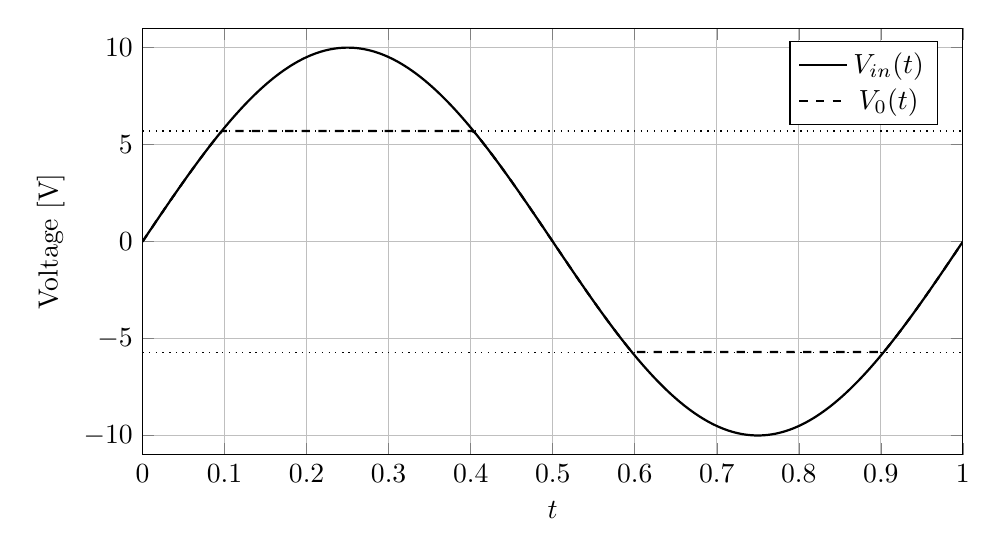
\begin{tikzpicture}
\begin{axis}[
    width=12cm,
    height=7cm,
    xlabel={$t$},
    ylabel={Voltage [V]},
    xmin=0, xmax=1,
    ymin=-11, ymax=11,
    grid=both,
    legend pos=north east,
    domain=0:1,
    samples=300
]

% Input voltage
\addplot[thick]
{10*sin(deg(2*pi*x))};
\addlegendentry{$V_{in}(t)$}

% Clipped output
\addplot[thick, dashed]
{
(10*sin(deg(2*pi*x)) > 5.7) * 5.7
+
(10*sin(deg(2*pi*x)) < -5.7) * (-5.7)
+
and(10*sin(deg(2*pi*x)) >= -5.7, 10*sin(deg(2*pi*x)) <= 5.7)
* (10*sin(deg(2*pi*x)))
};
\addlegendentry{$V_0(t)$}

% Reference lines
\addplot[dotted] {5.7};
\addplot[dotted] {-5.7};

\end{axis}
\end{tikzpicture}
\caption{$V_{in}(t)$ and $V_0(t)$}
\end{figure}
\clearpage
\noindent
With given that the max current is $110mA$, we can calculate what $R_1$ should be. We have already defined an expression for the maximum current and can set it equal to given value.
\[
I_{R1\uparrow} = \frac{10V - 5.7V}{R1}
\]
\[
110mA = \frac{10V - 5.7V}{R1}
\]
\[
R1 = 39\Omega
\]

\noindent
The total current is 0 whenever the input voltage is within $|V_0|<5.7V$.

\begin{figure}[H]
\centering
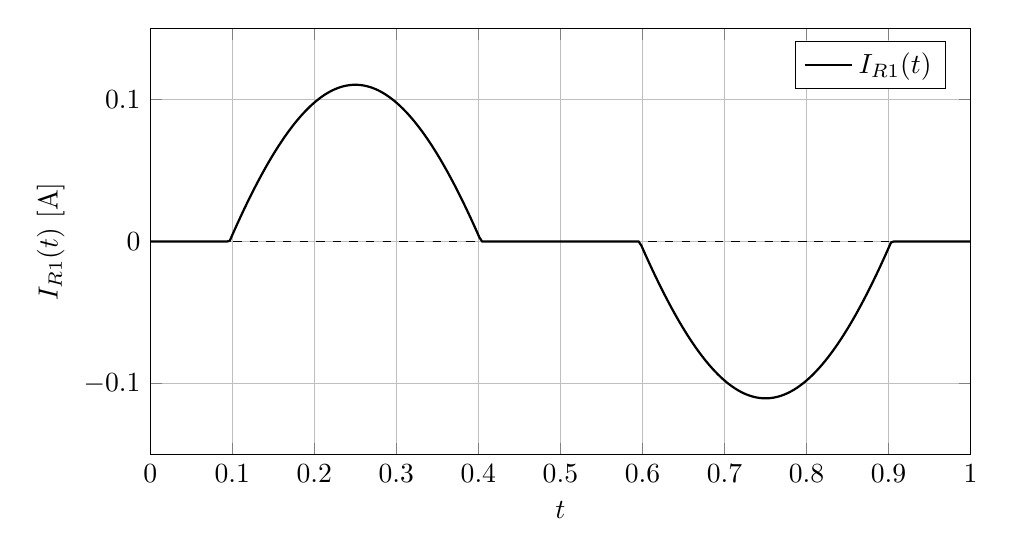
\begin{tikzpicture}
\begin{axis}[
    width=12cm,
    height=7cm,
    xlabel={$t$},
    ylabel={$I_{R1}(t)$ [A]},
    xmin=0, xmax=1,
    ymin=-0.15, ymax=0.15,
    grid=both,
    legend pos=north east,
    domain=0:1,
    samples=300
]

% Current
\addplot[thick]
{
(
(10*sin(deg(2*pi*x)) > 5.7)
* ((10*sin(deg(2*pi*x)) - 5.7)/39)
+
(10*sin(deg(2*pi*x)) < -5.7)
* ((10*sin(deg(2*pi*x)) + 5.7)/39)
)
};
\addlegendentry{$I_{R1}(t)$}

% Zero line
\addplot[dashed] {0};

\end{axis}
\end{tikzpicture}
\caption{Total current in the circuit.}
\end{figure}